\section{การวิเคราะห์ระบบ}

\subsection{วัสดุ อุปกรณ์ เครื่องมือที่ใช้พัฒนาและออกแบบระบบ}

\subsubsection{อุปกรณ์}

คอมพิวเตอร์ แท็บเล็ต

\subsubsection{เครื่องมือ}

\begin{itemize}
    \item Visual Studio Code
    \item Docker
    \item Laravel web framework
    \item Nuxt.js web framework
    \item draw.io
    \item Mermaid Chart
    \item Google Docs
\end{itemize}

\subsubsection{ระบบจัดการฐานข้อมูล}

MySQL

\subsection{Diagrams}

Diagram ต่าง ๆ ที่ถูกสร้างขึ้นในกระบวนการวิเคราะห์ระบบ

\subsubsection{Business Process ก่อนปรับปรุง}

\begin{figure}[!htb]
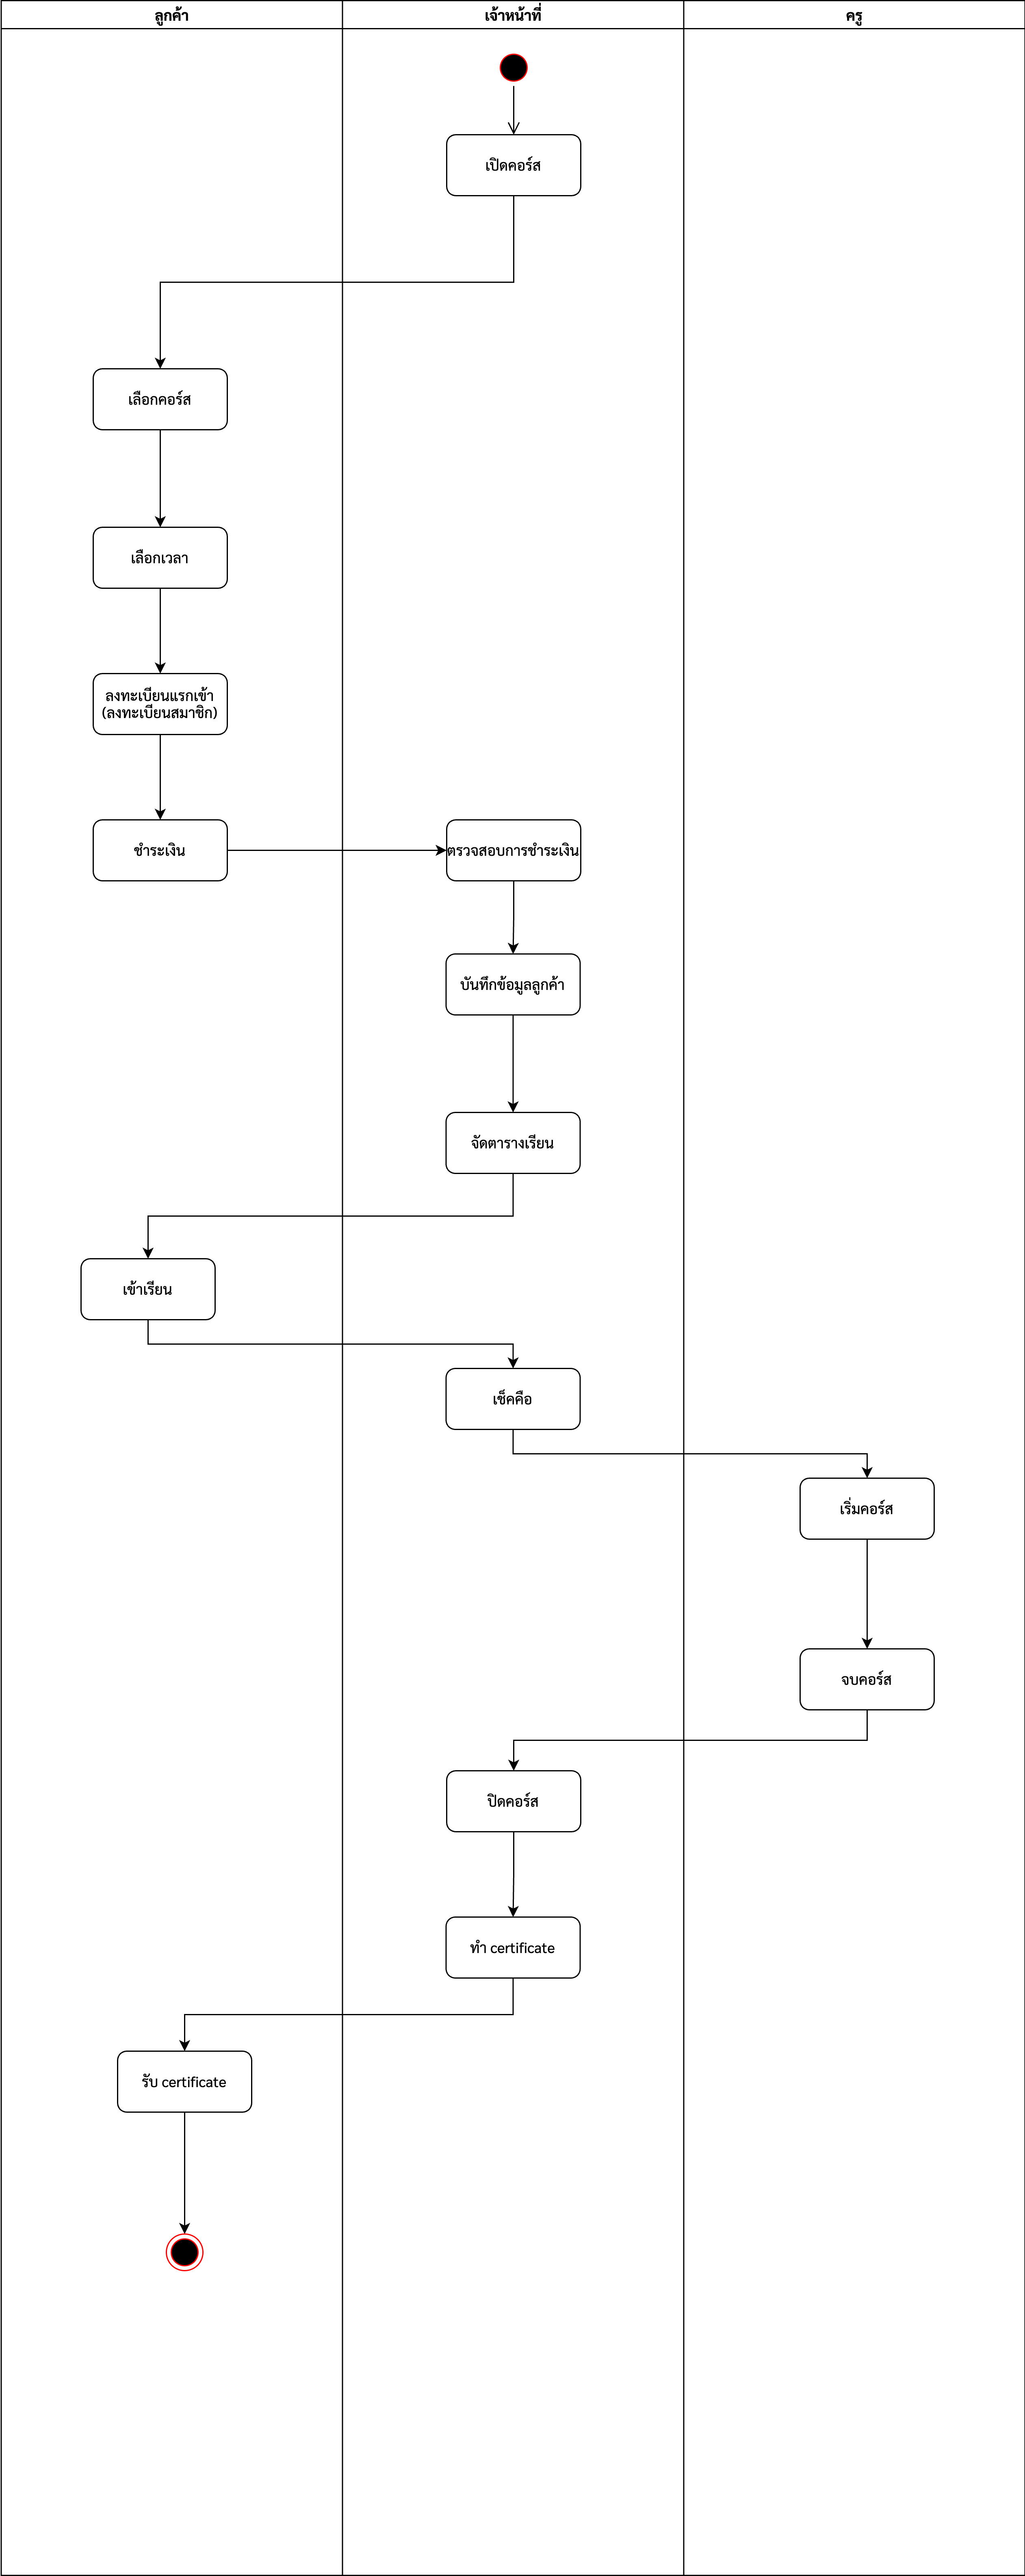
\includegraphics[width=\textwidth,height=0.95\textheight,keepaspectratio]{./figures/diagrams/activity/aqkids-activity-0.1.0.png}
\caption{Business Process ก่อนปรับปรุง}
\label{fig:aqkids-activity-draft}
\end{figure}

Business Process Digram ในรูปที่ \ref{fig:aqkids-activity-draft} แสดง Process ต่าง ๆ ของระบบ

\subsubsection{คำอธิบาย Business Process ก่อนปรับปรุง}

เจ้าหน้าที่เป็นผู้สร้างคอร์สเรียนเพื่อให้ลูกค้าสมัครเรียน คอร์สเรียนจำเป็นจะต้องมีครูผู้รับผิดชอบคอร์ส โดยครูจะต้องผ่านการประเมินคุณสมบัติ เมื่อผ่านจึงจะเป็นผู้รับผิดชอบคอร์สได้ เมื่อสร้างคอร์สสำเร็จ ลูกค้าจะสมัครคอร์สโดยขั้นตอนมีดังนี้

\begin{enumerate}
    \item เลือกเวลาที่ต้องการสมัครคอร์สเรียน
    \item ชำระเงินค่าคอร์สเรียน
\end{enumerate}

เมื่อลูกค้าชำระเงินค่าคอร์สเรียนสำเร็จ เจ้าหน้าที่จะตรวจสอบหลักฐานการชำระเงินค่าเรียน เมื่อตรวจสอบแล้วพบว่าลูกค้าชำระเงินแล้วจริง เจ้าหน้าที่จะจัดตารางเรียนให้ลูกค้า เมื่อลูกค้าสมัครคอร์สจนครบตามจำนวนที่คอร์สรับได้ ครูจะยืนยันการรับผิดชอบคอร์ส

เมื่อถึงเวลาของคาบเรียนแรก จะถือว่าคอร์สเรียนได้เริ่มขึ้น ในทุก ๆ คาบเรียน ครูจะมีหน้าที่

\begin{enumerate}
    \item ลงชื่อเข้าสอนด้วยตนเอง
    \item รายงานการเข้าเรียนของลูกค้าทุกคนในแต่ละคาบเรียน
\end{enumerate}

ในกรณีที่ครูหรือลูกค้าคนใดไม่สามารถเข้าสอนหรือเข้าเรียนได้ เจ้าหน้าที่มีหน้าที่จัดหาคาบเรียนเพื่อให้ลูกค้าเรียนชดเชยร่วมกับคาบเรียนอื่น หากไม่สามารถจัดหาได้ จะต้องจองคาบเรียนชดเชยให้กับลูกค้าคนนั้น

เมื่อลูกค้าทุกคนที่สมัครเรียนคอร์สเรียนครบตามจำนวนครั้งที่คอร์สกำหนดจะถือว่าคอร์สเรียนได้จบลง
หลังจากที่คอร์สเรียนจบลง เจ้าหน้าที่จะมีหน้าที่ 3 หน้าที่ ดังนี้

\begin{enumerate}
    \item จัดทำใบประกาศนีย์บัตรให้กับลูกค้า
    \item จ่ายเงินค่าทำงานให้กับครูผู้รับผิดชอบคอร์ส
    \item จัดทำรายงานการเงินของคอร์ส
\end{enumerate}

\subsubsection{Business Process ที่ปรับปรุงแล้ว}

\begin{figure}[H]
\includegraphics[width=\textwidth,height=0.95\textheight,keepaspectratio]{./figures/diagrams/activity/aqkids-activity-2.0.0-splitted-top.png}
\caption{Business Process ที่ปรับปรุงแล้ว (1 จาก 2)}
\label{fig:aqkids-activity-final-1}
\end{figure}

\begin{figure}[H]
\includegraphics[width=\textwidth,height=0.95\textheight,keepaspectratio]{./figures/diagrams/activity/aqkids-activity-2.0.0-splitted-bottom.png}
\caption{Business Process ที่ปรับปรุงแล้ว (1 จาก 2)}
\label{fig:aqkids-activity-final-2}
\end{figure}

% รูปที่ \ref{fig:aqkids-activity-final-1} และ \ref{fig:aqkids-activity-final-2} แสดง Business Process ที่ปรับปรุงแล้ว \marginpar{\includegraphics[width=\marginparwidth]{./figures/diagrams/activity/aqkids-activity-2.0.0-splitted-top.png}}

\subsubsection{คำอธิบาย Business Process ที่ปรับปรุงแล้ว}
เจ้าหน้าที่ ครู และลูกค้า จะเป็นจะต้องมีบัญชีผู้ใช้ของระบบ โดยการสร้างบัญชีผู้ใช้ของระบบจะมีเงื่อนไขดังนี้

\begin{minipage}{\textwidth}
\begin{enumerate}
    \item บัญชีผู้ใช้ระบบของเจ้าหน้าที่จะมีให้โดยปริยายตั้งแต่ส่งมอบระบบ
    \item บัญชีผู้ใช้ระบบของครูจะถูกสร้างโดยเจ้าหน้าที่
    \item ลูกค้าสามารถสร้างบัญชีผู้ใช้ของระบบได้ด้วยตนเอง
\end{enumerate}
\end{minipage}

เจ้าหน้าที่เป็นผู้สร้างคอร์สเรียนเพื่อให้ลูกค้าสมัครเรียน คอร์สเรียนจำเป็นจะต้องมีครูผู้รับผิดชอบคอร์สซึ่งจะถูกมอบความรับผิดชอบโดยเจ้าหน้าที่ เมื่อคอร์สเรียนถูกสร้าง เจ้าหน้าที่จะจองเวลาเรียนของคอร์ส

\begin{minipage}{\textwidth}
ลูกค้าจะสมัครคอร์สโดยขั้นตอนมีดังนี้

\begin{enumerate}
    \item เลือกเวลาที่ต้องการสมัครคอร์สเรียน
    \item ชำระเงินค่าคอร์สเรียน
    \item อัปโหลดหลักฐานการชำระเงินค่าคอร์สและกดยืนยันภายใน 5 นาที
    \begin{itemize}
        \item หากทันเวลาจะถือว่าสร้างคำขอการสมัครคอร์สเรียนสำเร็จ
        \item หากไม่ทันเวลา ลูกค้าสามารถส่งคำขอคืนเงินได้ โดยอัปโหลดหลักฐานการโอนเงิน
    \end{itemize}
\end{enumerate}
\end{minipage}

ทั้งคำขอการสมัครคอร์สเรียนและคำขอคืนเงินจะถูกตรวจสอบหลักฐานโดยเจ้าหน้าที่ หากตรวจสอบพบว่าหลักฐานไม่ถูกต้องคำขอจะถูกละทิ้ง (Abort) แต่หากตรวจสอบแล้วพบว่าถูกต้อง เจ้าหน้าที่จะอนุมัติคำขอสมัครเรียนและออกใบเสร็จรับเงินค่าสมัครคอร์สเรียนให้สำหรับคำขอการสมัครคอร์สเรียน และอนุมัติคำขอคืนเงินสำหรับคำขอคืนเงิน

เมื่อถึงเวลาของคาบเรียนแรก จะถือว่าคอร์สเรียนได้เริ่มขึ้น ในทุก ๆ คาบเรียน ครูจะมีหน้าที่
ลงชื่อเข้าสอนด้วยตนเอง และรายงานการเข้าเรียนของลูกค้าทุกคนในแต่ละคาบเรียน

ในกรณีที่ครูหรือลูกค้าคนใดไม่สามารถเข้าสอนหรือเข้าเรียนได้ เจ้าหน้าที่มีหน้าที่จัดหาคาบเรียนเพื่อให้ลูกค้าเรียนชดเชยร่วมกับคาบเรียนอื่น หากไม่สามารถจัดหาได้ จะต้องจองคาบเรียนชดเชยให้กับลูกค้าคนนั้น

เมื่อลูกค้าทุกคนที่สมัครเรียนคอร์สเรียนครบตามจำนวนครั้งที่คอร์สกำหนดจะถือว่าคอร์สเรียนได้จบลง
หลังจากที่คอร์สเรียนจบลง เจ้าหน้าที่จะมีหน้าที่จัดทำใบประกาศนีย์บัตรให้กับลูกค้า

\subsubsection{Business Process ที่สัมพันธ์กับ Use Case}

\begin{figure}[H]
\includegraphics[width=\textwidth,height=0.95\textheight,keepaspectratio]{./figures/diagrams/activity/aqkids-activity-2.0.0-uc-splitted-top.png}
\caption{Business Process ที่ปรับปรุงแล้ว (1 จาก 2)}
\label{fig:aqkids-activity-uc-final-1}
\end{figure}

\begin{figure}[H]
\includegraphics[width=\textwidth,height=0.95\textheight,keepaspectratio]{./figures/diagrams/activity/aqkids-activity-2.0.0-uc-splitted-bottom.png}
\caption{Business Process ที่ปรับปรุงแล้ว (2 จาก 2)}
\label{fig:aqkids-activity-uc-final-2}
\end{figure}

% รูปที่ \ref{fig:aqkids-activity-uc-final-1} และ \ref{fig:aqkids-activity-uc-final-2} แสดง Business Process ที่สัมพันธ์กับ Use Case \marginpar{\includegraphics[width=\marginparwidth]{./figures/diagrams/activity/aqkids-activity-2.0.0-uc-splitted-top.png}}

\subsubsection{ตารางจับคู่ระหว่าง Business Process ID และ Use Case ID}

\begin{table}[H]
\caption{ตารางจับคู่ระหว่าง Business Process ID และ Use Case ID}
\label{tab:bp-uc-mapping}
\begin{tabularx}{\textwidth}{|X|X|}
\hline
\multicolumn{1}{|X|}{\textbf{Business Process ID}} & \multicolumn{1}{c|}{\textbf{Use Case ID}} \\ \hline
1  & 1 \\ \hline
2  & 1 \\ \hline
3  & 1 \\ \hline
4  & 1 \\ \hline
5  & 2 \\ \hline
6  & 2 \\ \hline
7  & 2 \\ \hline
8  & 3 \\ \hline
9  & 4 \\ \hline
10 & 4 \\ \hline
11 & 4 \\ \hline
12 & 4 \\ \hline
13 & 4 \\ \hline
14 & 4 \\ \hline
15 & 4 \\ \hline
16 & 5 \\ \hline
17 & 5 \\ \hline
18 & 6 \\ \hline
19 & 7 \\ \hline
20 & 7 \\ \hline
21 & 7 \\ \hline
\end{tabularx}
\end{table}

\subsubsection{Use Case Diagram ก่อนปรับปรุง}

\begin{figure}[H]
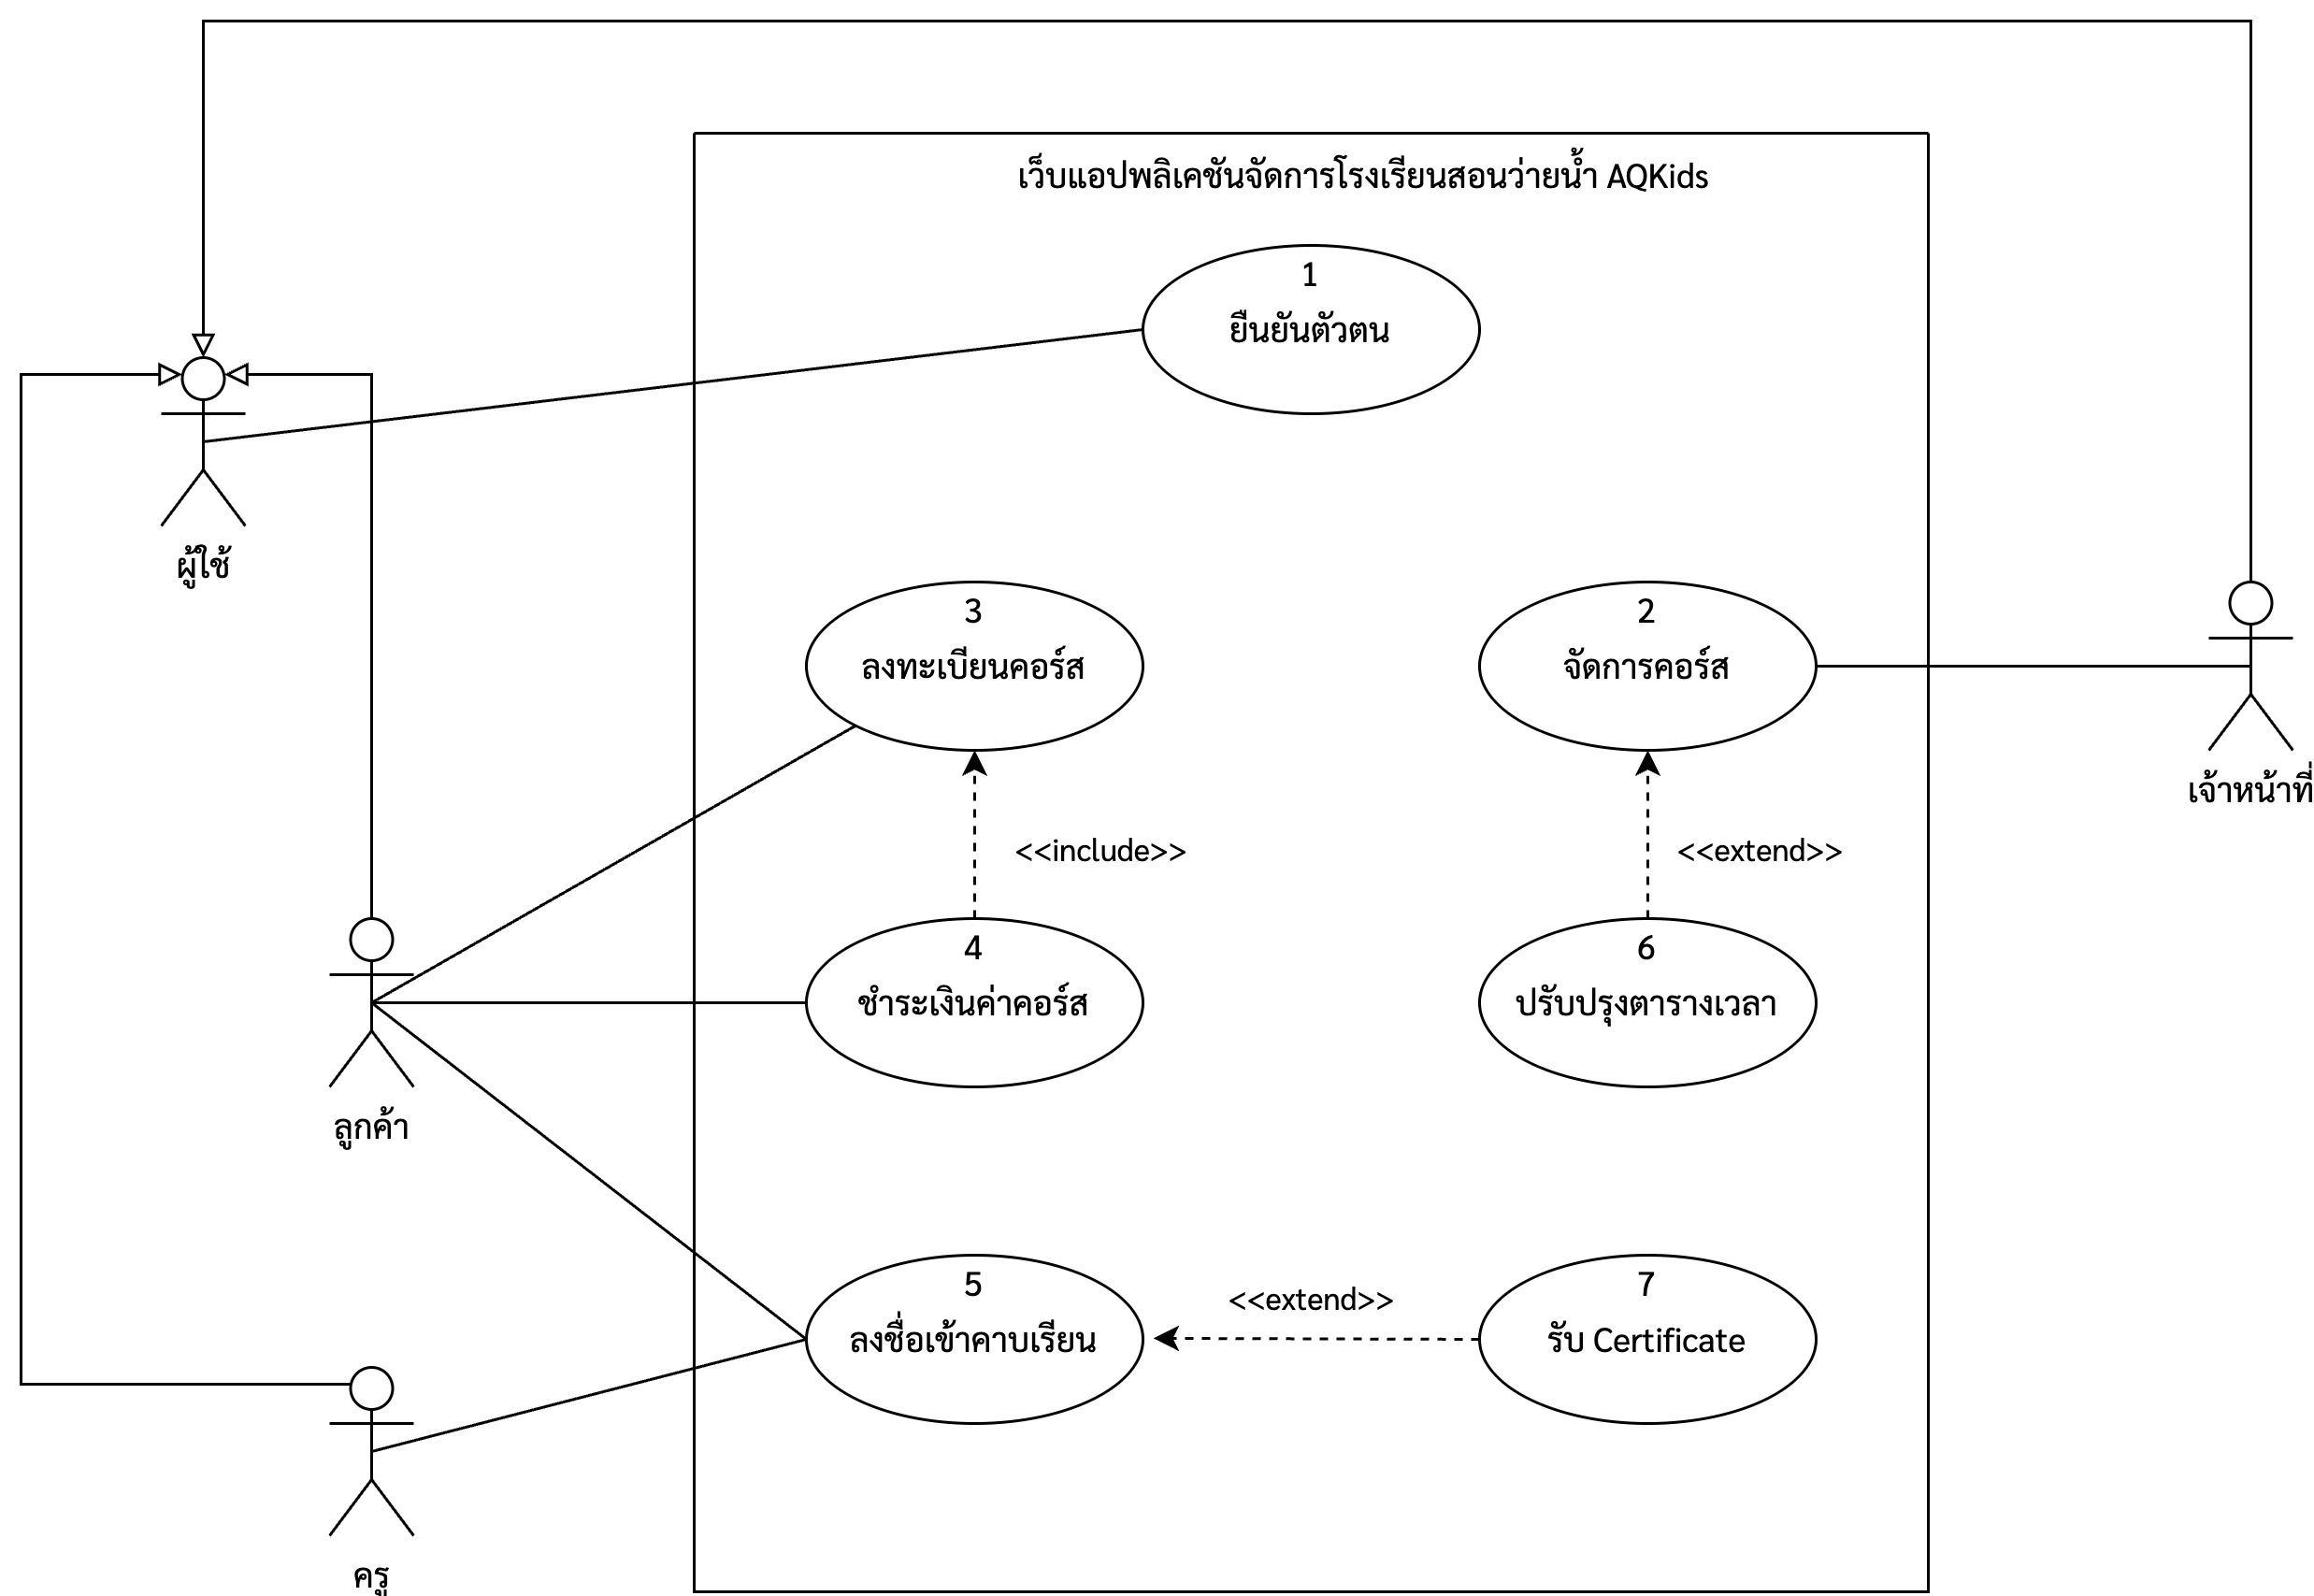
\includegraphics[width=\textwidth,height=0.95\textheight,keepaspectratio]{./figures/diagrams/use-case/aqkids-use-case-0.1.0.png}
\caption{Use Case Diagram ก่อนปรับปรุง}
\label{fig:aqkids-use-case-draft}
\end{figure}

% รูปที่ \ref{fig:aqkids-use-case-draft} แสดง Use Case Diagram ก่อนปรับปรุง

\begin{landscape}
\subsubsection{CRUD Table}

\begin{table}[H]
\caption{CRUD Table}
\label{tab:crud-table-draft}
\begin{tabularx}{\textwidth}{|l|X|X|X|l|X|l|X|l|}
\hline
\multicolumn{1}{|X|}{\textbf{VC}} & \textbf{users} & \textbf{courses}      & \textbf{enrollments}  & \multicolumn{1}{c|}{\textbf{receipts}} & \textbf{timeslots}    & \multicolumn{1}{c|}{\textbf{teacher\_attendances}} & \textbf{student\_attendances} & \multicolumn{1}{c|}{\textbf{user\_requests}} \\ \hline
\textbf{ยืนยันตัวตน}              & CRU            & \multicolumn{1}{l|}{} & \multicolumn{1}{l|}{} &                                        & \multicolumn{1}{l|}{} &                                                    & \multicolumn{1}{l|}{}         &                                              \\ \hline
\textbf{จัดการคอร์ส}              & R              & CRU                   & \multicolumn{1}{l|}{} &                                        & CR                    & \multicolumn{1}{c|}{CR}                            & \multicolumn{1}{l|}{}         &                                              \\ \hline
\textbf{สมัครคอร์ส}               & R              & R                     & CR                    &                                        & \multicolumn{1}{l|}{} &                                                    & \multicolumn{1}{l|}{}         &                                              \\ \hline
\textbf{จัดการการชำระค่าคอร์ส}    & R              & R                     & RU                    & \multicolumn{1}{c|}{CR}                & \multicolumn{1}{l|}{} &                                                    & CR                            & \multicolumn{1}{c|}{CRU}                     \\ \hline
\textbf{ลงชื่อเข้าคาบเรียน}       & R              & R                     & R                     &                                        & R                     & \multicolumn{1}{c|}{RU}                            & RU                            &                                              \\ \hline
\textbf{ปรับปรุงตารางเวลา}        & R              & R                     & R                     &                                        & CRD                   & \multicolumn{1}{c|}{CRD}                           & CRD                           &                                              \\ \hline
\textbf{รับ Certificate}          & R              & R                     & R                     &                                        & R                     &                                                    & R                             &                                              \\ \hline
\end{tabularx}
\end{table}
\end{landscape}

\subsubsection{คำอธิบายประกอบ CRUD Table}

\begin{table}[H]
\caption{คำอธิบายประกอบ CRUD Table}
\label{tab:crud-description}
\begin{tabularx}{\textwidth}{|ll|}
\hline
\multicolumn{2}{|l|}{Use Case 1: ยืนยันตัวตน}                                                                    \\ \hline
\multicolumn{1}{|l|}{Read}  & users                                                                              \\ \hline
\multicolumn{1}{|l|}{Write} & users                                                                              \\ \hline
\multicolumn{2}{|l|}{Use Case 2: จัดการคอร์ส}                                                                    \\ \hline
\multicolumn{1}{|l|}{Read}  & users, courses, timeslots, teacher\_attendances                                    \\ \hline
\multicolumn{1}{|l|}{Write} & courses, timeslots, teacher\_attendances                                           \\ \hline
\multicolumn{2}{|l|}{Use Case 3: สมัครคอร์ส}                                                                     \\ \hline
\multicolumn{1}{|l|}{Read}  & users, courses, enrollments                                                        \\ \hline
\multicolumn{1}{|l|}{Write} & enrollments                                                                        \\ \hline
\multicolumn{2}{|l|}{Use Case 4: จัดการการชำระค่าคอร์ส}                                                          \\ \hline
\multicolumn{1}{|l|}{Read}  & users, courses, enrollments, receipts, student\_attendances, user\_requests        \\ \hline
\multicolumn{1}{|l|}{Write} & receipts, student\_attendances, user\_requests                                     \\ \hline
\multicolumn{2}{|l|}{Use Case 5: ลงชื่อเข้าคาบเรียน}                                                             \\ \hline
\multicolumn{1}{|l|}{Read}  & users, courses, enrollments, timeslots, teacher\_attendances, student\_attendances \\ \hline
\multicolumn{1}{|l|}{Write} & teacher\_attendances, student\_attendances                                         \\ \hline
\multicolumn{2}{|l|}{Use Case 6: ปรับปรุงตารางเวลา}                                                              \\ \hline
\multicolumn{1}{|l|}{Read}  & users, courses, enrollments, timeslots, teacher\_attendances, student\_attendances \\ \hline
\multicolumn{1}{|l|}{Write} & timeslots, teacher\_attendances, student\_attendances                              \\ \hline
\multicolumn{2}{|l|}{Use Case 7: รับ Certificate}                                                                \\ \hline
\multicolumn{1}{|l|}{Read}  & users, courses, enrollments, timeslots, student\_attendances                       \\ \hline
\multicolumn{1}{|l|}{Write} & -                                                                                  \\ \hline
\end{tabularx}
\end{table}

\subsubsection{Use Case Diagram ที่ผ่านการทบทวนปรับปรุงแล้ว}

\begin{figure}[H]
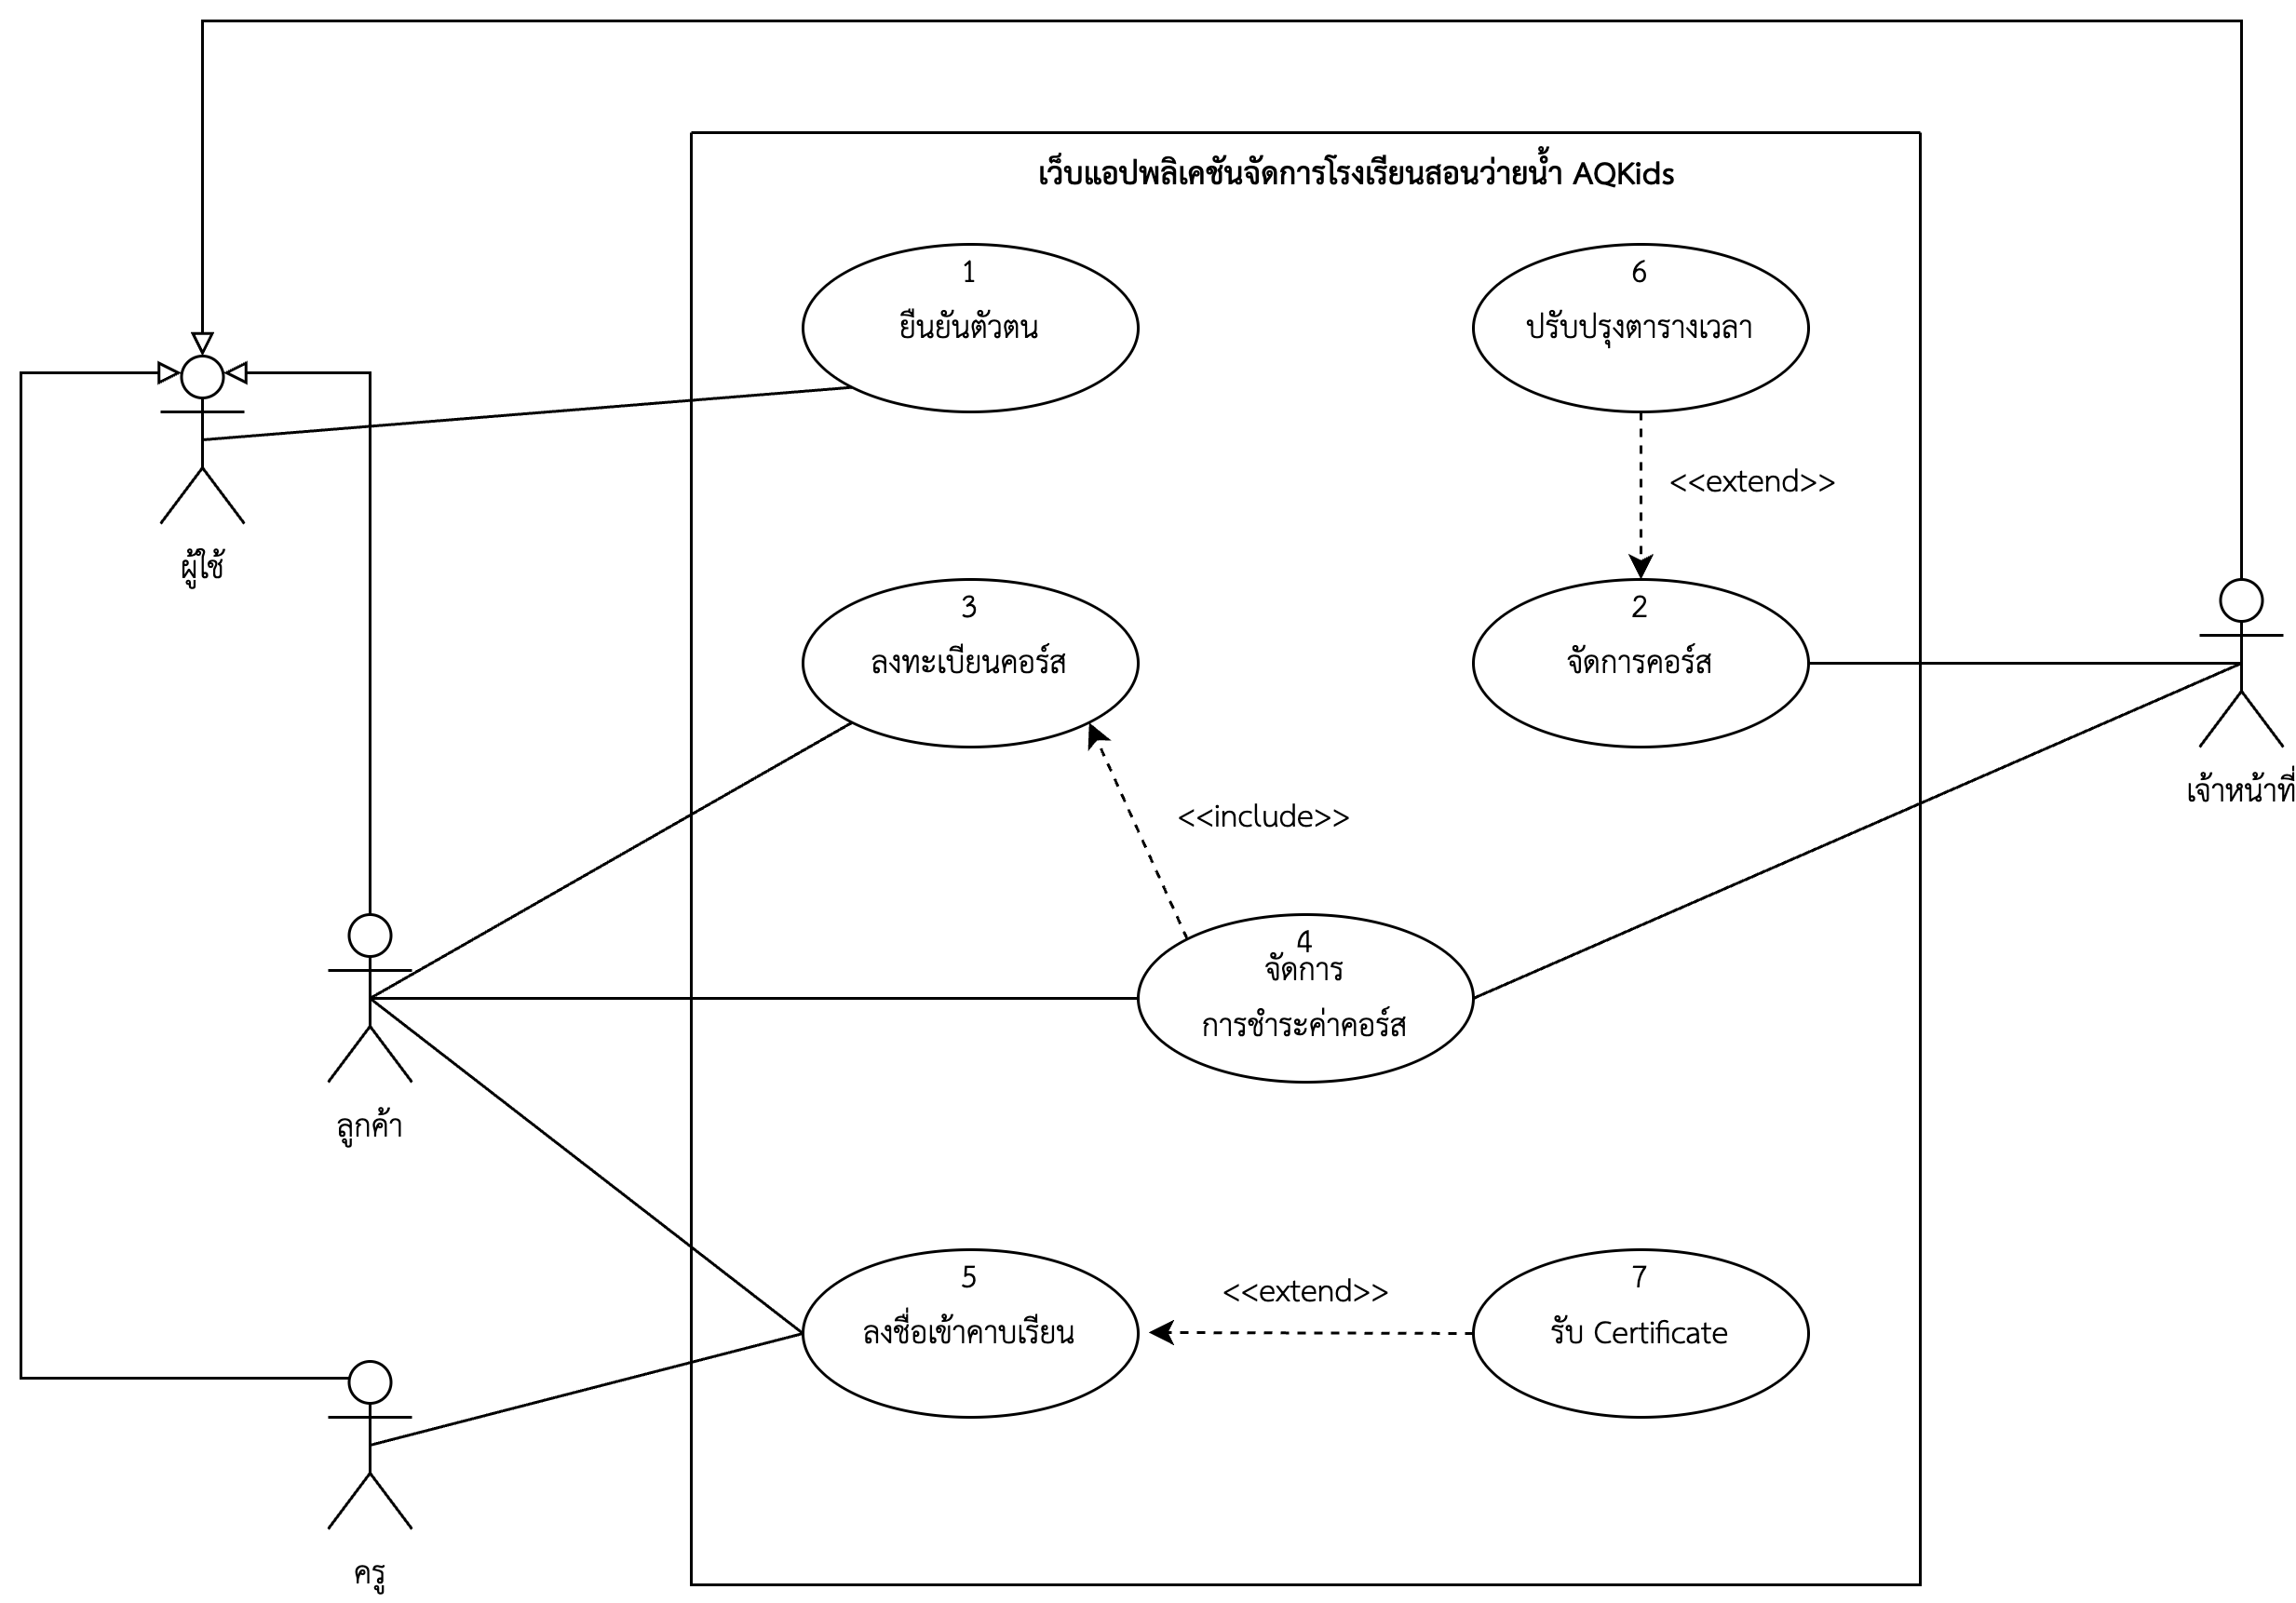
\includegraphics[width=\textwidth,height=0.95\textheight,keepaspectratio]{./figures/diagrams/use-case/aqkids-use-case-1.0.0.png}
\caption{Use Case Diagram ที่ผ่านการทบทวนปรับปรุงแล้ว}
\label{fig:aqkids-use-case-final}
\end{figure}

% รูปที่ \ref{fig:aqkids-use-case-final} แสดง Use Case Diagram ที่ผ่านการทบทวนปรับปรุงแล้ว % \marginpar{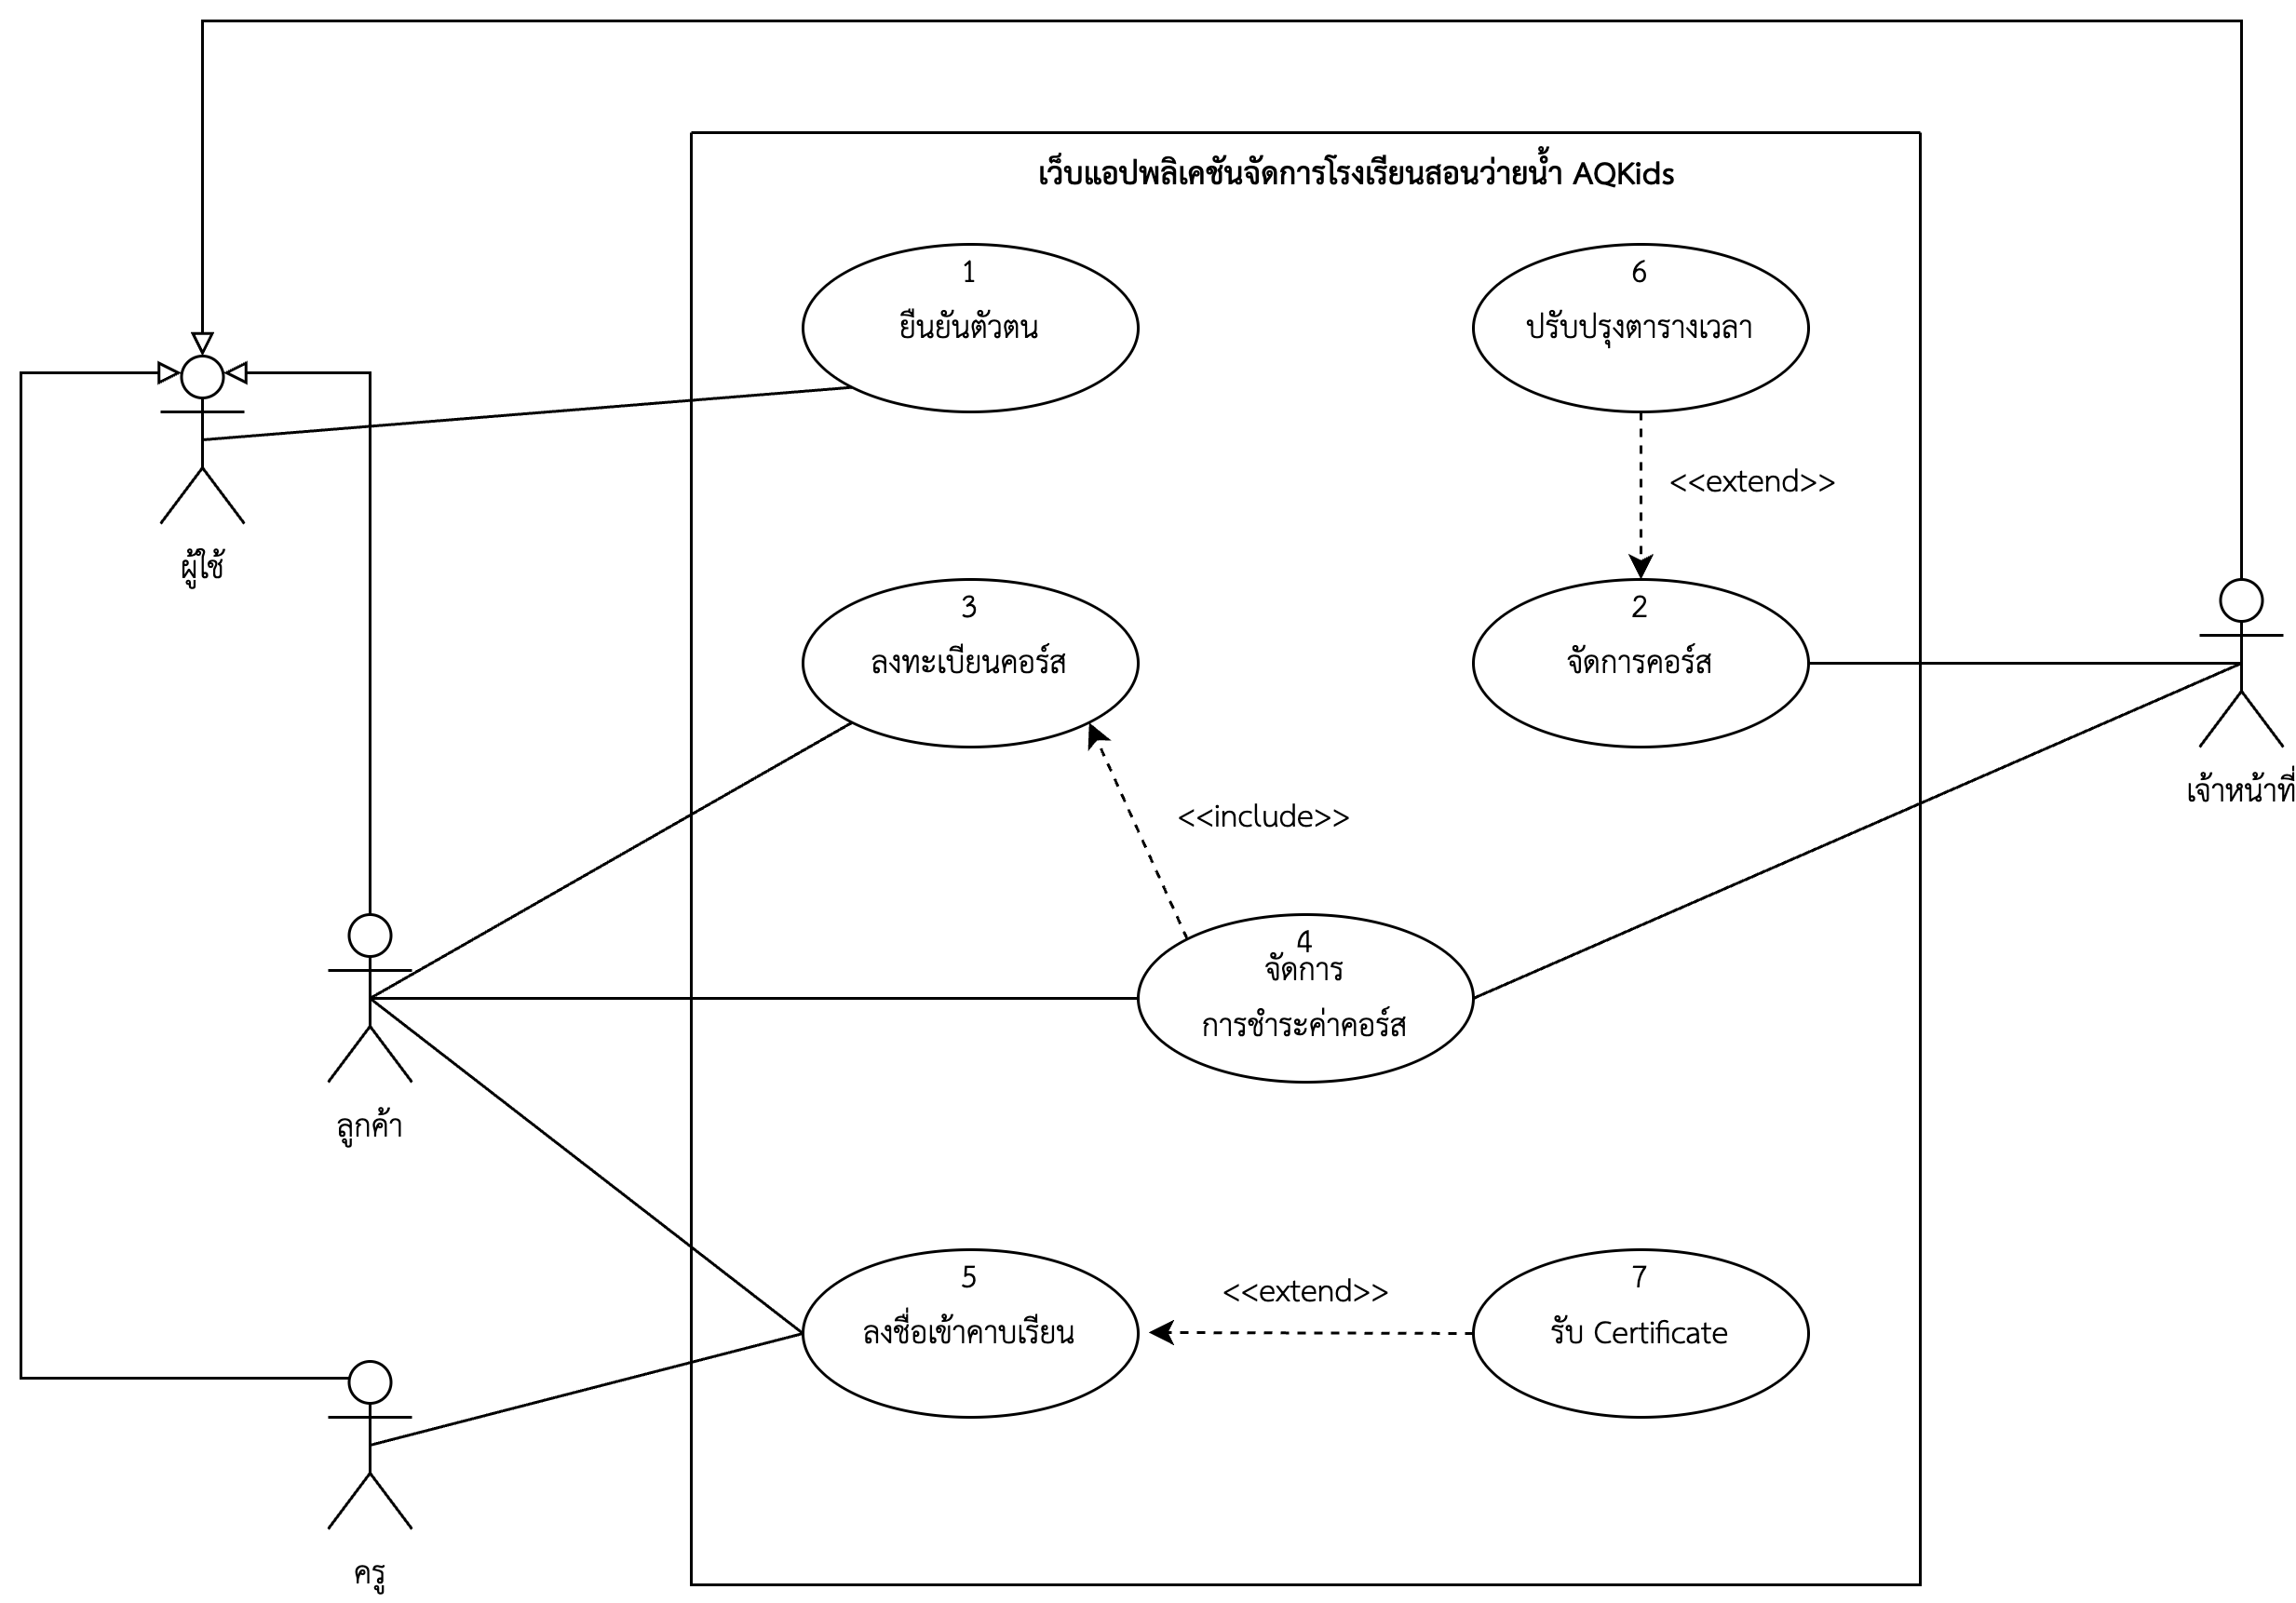
\includegraphics[width=\marginparwidth]{./figures/diagrams/use-case/aqkids-use-case-1.0.0.png}}

\begin{landscape}
\subsubsection{CRUD Table ที่ผ่านการทบทวนแล้ว}

\begin{table}[H]
\caption{CRUD Table ที่ผ่านการทบทวนแล้ว}
\label{tab:crud-table-draft}
\begin{tabularx}{\textwidth}{|l|X|X|X|l|X|l|X|l|}
\hline
\multicolumn{1}{|X|}{\textbf{VC}} & \textbf{users} & \textbf{courses}      & \textbf{enrollments}  & \multicolumn{1}{c|}{\textbf{receipts}} & \textbf{timeslots}    & \multicolumn{1}{c|}{\textbf{teacher\_attendances}} & \textbf{student\_attendances} & \multicolumn{1}{c|}{\textbf{user\_requests}} \\ \hline
\textbf{ยืนยันตัวตน}              & CRU            & \multicolumn{1}{l|}{} & \multicolumn{1}{l|}{} &                                        & \multicolumn{1}{l|}{} &                                                    & \multicolumn{1}{l|}{}         &                                              \\ \hline
\textbf{จัดการคอร์ส}              & R              & CRU                   & \multicolumn{1}{l|}{} &                                        & CR                    & \multicolumn{1}{c|}{CR}                            & \multicolumn{1}{l|}{}         &                                              \\ \hline
\textbf{สมัครคอร์ส}               & R              & R                     & CR                    &                                        & \multicolumn{1}{l|}{} &                                                    & \multicolumn{1}{l|}{}         &                                              \\ \hline
\textbf{จัดการการชำระค่าคอร์ส}    & R              & R                     & RU                    & \multicolumn{1}{c|}{CR}                & \multicolumn{1}{l|}{} &                                                    & CR                            & \multicolumn{1}{c|}{CRU}                     \\ \hline
\textbf{ลงชื่อเข้าคาบเรียน}       & R              & R                     & R                     &                                        & R                     & \multicolumn{1}{c|}{RU}                            & RU                            &                                              \\ \hline
\textbf{ปรับปรุงตารางเวลา}        & R              & R                     & R                     &                                        & CRD                   & \multicolumn{1}{c|}{CRD}                           & CRD                           &                                              \\ \hline
\textbf{รับ Certificate}          & R              & R                     & R                     &                                        & R                     &                                                    & R                             &                                              \\ \hline
\end{tabularx}
\end{table}
\end{landscape}

\subsubsection{คำอธิบายประกอบ CRUD Table ที่ผ่านการทบทวนแล้ว}

\begin{table}[H]
\caption{คำอธิบายประกอบ CRUD Table ที่ผ่านการทบทวนแล้ว}
\label{tab:crud-description-final}
\begin{tabularx}{\textwidth}{|ll|}
\hline
\multicolumn{2}{|l|}{Use Case 1: ยืนยันตัวตน}                                                                    \\ \hline
\multicolumn{1}{|l|}{Read}  & users                                                                              \\ \hline
\multicolumn{1}{|l|}{Write} & users                                                                              \\ \hline
\multicolumn{2}{|l|}{Use Case 2: จัดการคอร์ส}                                                                    \\ \hline
\multicolumn{1}{|l|}{Read}  & users, courses, timeslots, teacher\_attendances                                    \\ \hline
\multicolumn{1}{|l|}{Write} & courses, timeslots, teacher\_attendances                                           \\ \hline
\multicolumn{2}{|l|}{Use Case 3: สมัครคอร์ส}                                                                     \\ \hline
\multicolumn{1}{|l|}{Read}  & users, courses, enrollments                                                        \\ \hline
\multicolumn{1}{|l|}{Write} & enrollments                                                                        \\ \hline
\multicolumn{2}{|l|}{Use Case 4: จัดการการชำระค่าคอร์ส}                                                          \\ \hline
\multicolumn{1}{|l|}{Read}  & users, courses, enrollments, receipts, student\_attendances, user\_requests        \\ \hline
\multicolumn{1}{|l|}{Write} & receipts, student\_attendances, user\_requests                                     \\ \hline
\multicolumn{2}{|l|}{Use Case 5: ลงชื่อเข้าคาบเรียน}                                                             \\ \hline
\multicolumn{1}{|l|}{Read}  & users, courses, enrollments, timeslots, teacher\_attendances, student\_attendances \\ \hline
\multicolumn{1}{|l|}{Write} & teacher\_attendances, student\_attendances                                         \\ \hline
\multicolumn{2}{|l|}{Use Case 6: ปรับปรุงตารางเวลา}                                                              \\ \hline
\multicolumn{1}{|l|}{Read}  & users, courses, enrollments, timeslots, teacher\_attendances, student\_attendances \\ \hline
\multicolumn{1}{|l|}{Write} & timeslots, teacher\_attendances, student\_attendances                              \\ \hline
\multicolumn{2}{|l|}{Use Case 7: รับ Certificate}                                                                \\ \hline
\multicolumn{1}{|l|}{Read}  & users, courses, enrollments, timeslots, student\_attendances                       \\ \hline
\multicolumn{1}{|l|}{Write} & -                                                                                  \\ \hline
\end{tabularx}
\end{table}

\subsubsection{ER Diagram}

\begin{figure}[H]
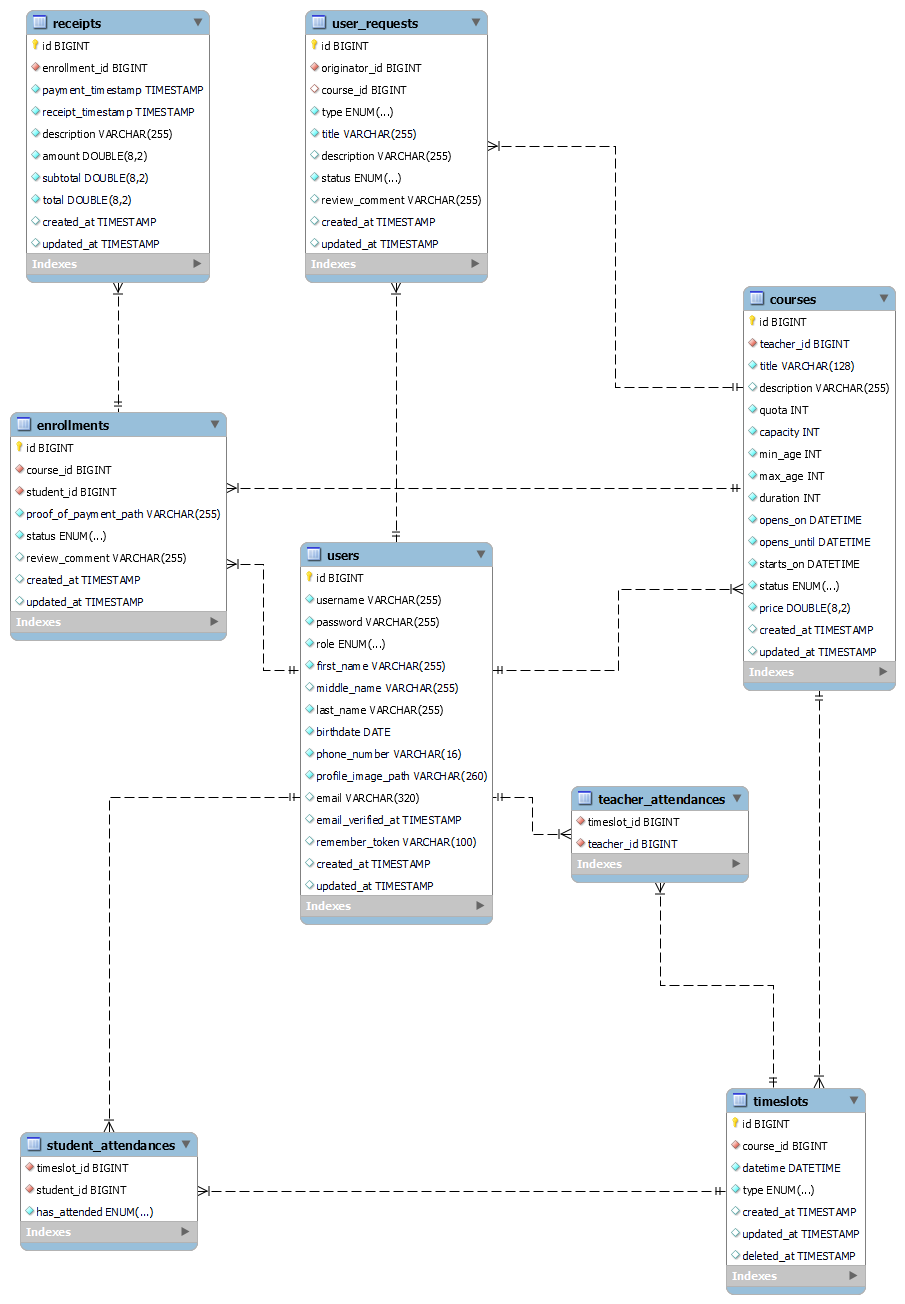
\includegraphics[width=\textwidth,height=0.95\textheight,keepaspectratio]{./figures/diagrams/entity-relationship/aqkids-entity-relationship-1.0.0.png}
\caption{ER Diagram}
\label{fig:aqkids-entity-relationship}
\end{figure}

% รูปที่ \ref{fig:aqkids-entity-relationship} แสดง ER Diagram % \marginpar{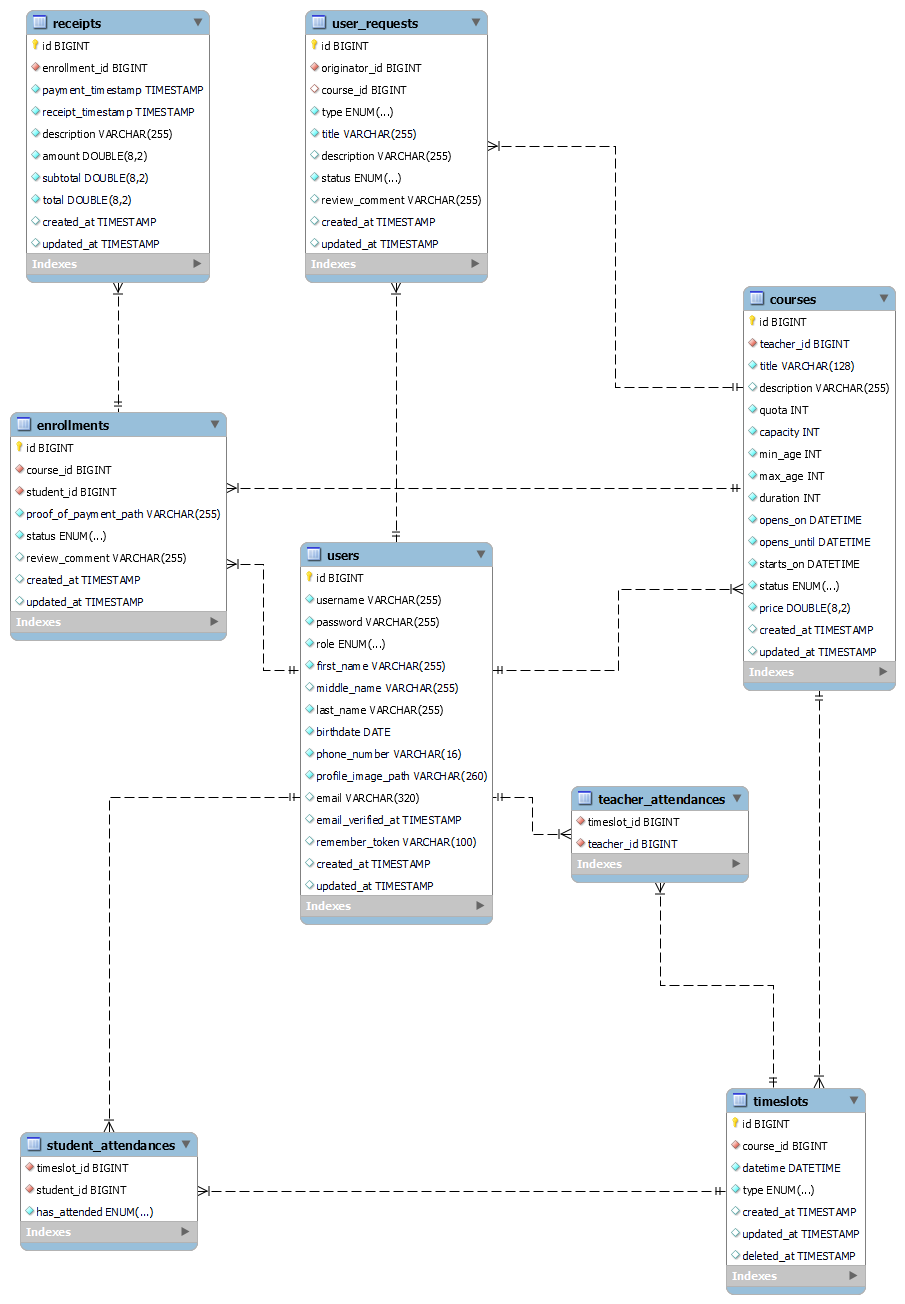
\includegraphics[width=\marginparwidth]{./figures/diagrams/entity-relationship/aqkids-entity-relationship-1.0.0.png}}

\subsubsection{ER Diagram พร้อม MySQL Queries ประกอบ}

\begin{figure}[H]
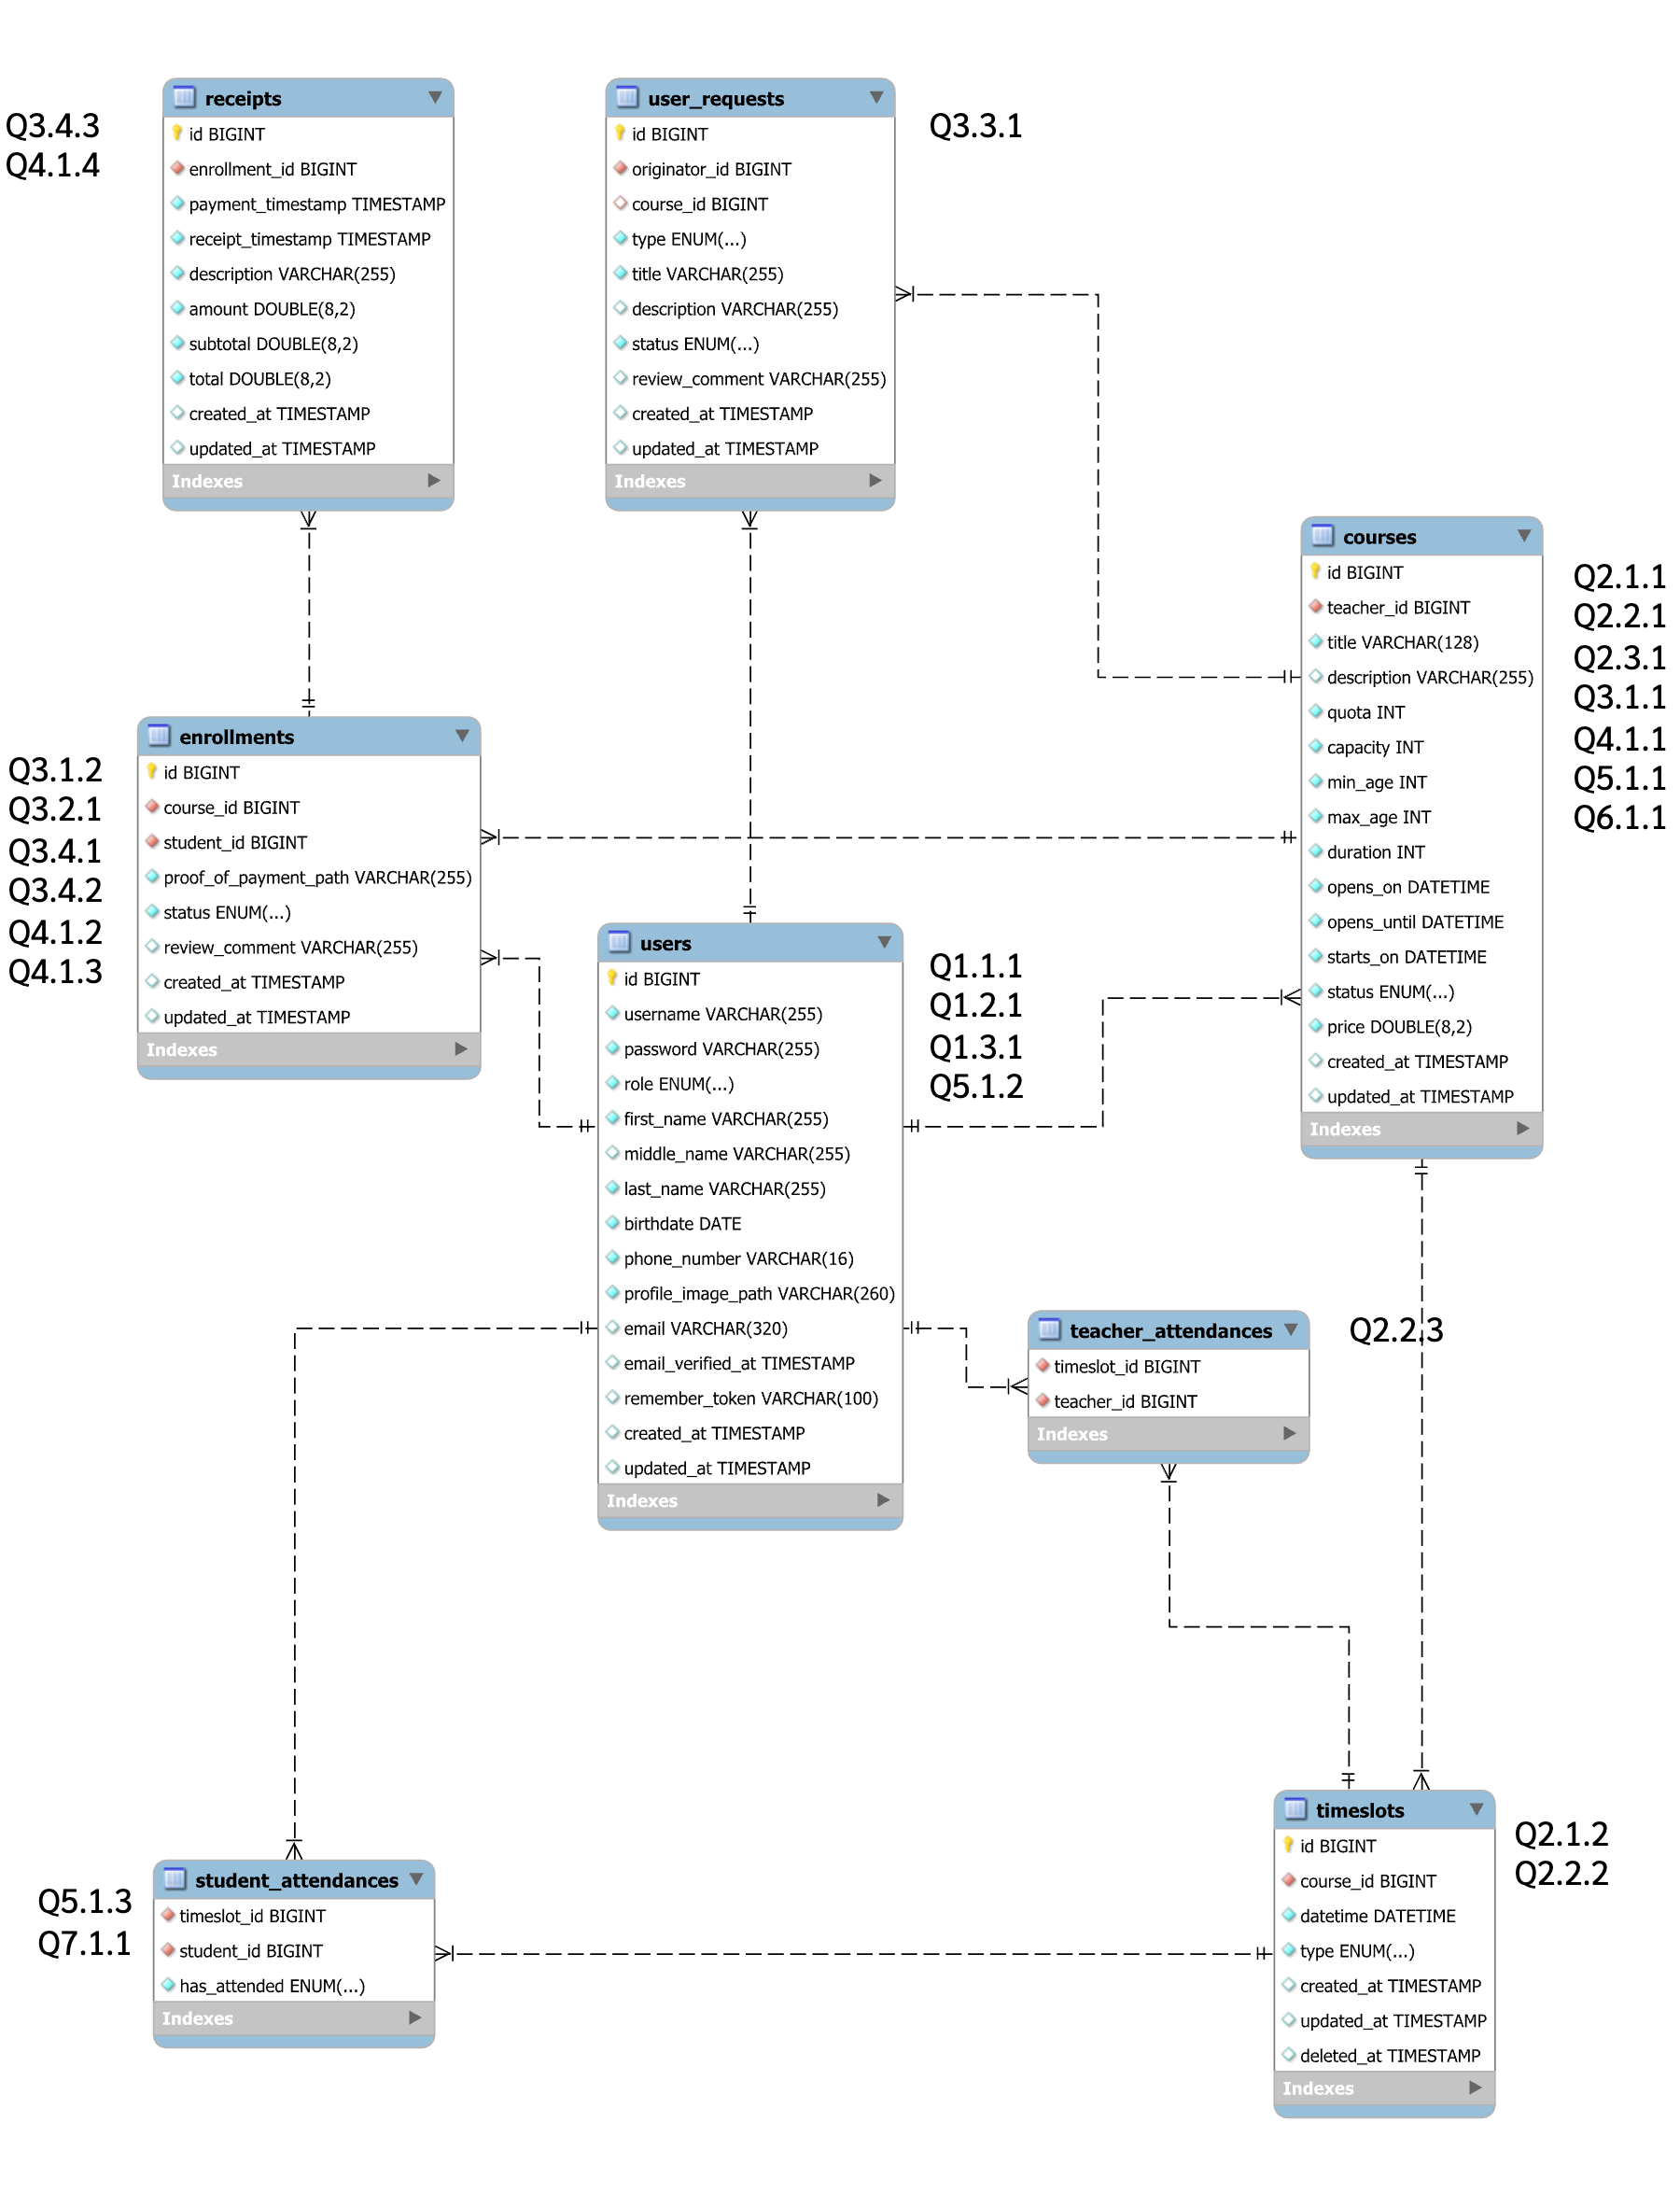
\includegraphics[width=\textwidth,height=0.95\textheight,keepaspectratio]{./figures/diagrams/entity-relationship/aqkids-entity-relationship-1.0.0-queries.png}
\caption{ER Diagram พร้อม MySQL Queries ประกอบ}
\label{fig:aqkids-entity-relationship-queries}
\end{figure}

% รูปที่ \ref{fig:aqkids-entity-relationship-queries} แสดง ER Diagram พร้อม MySQL Queries ประกอบ % \marginpar{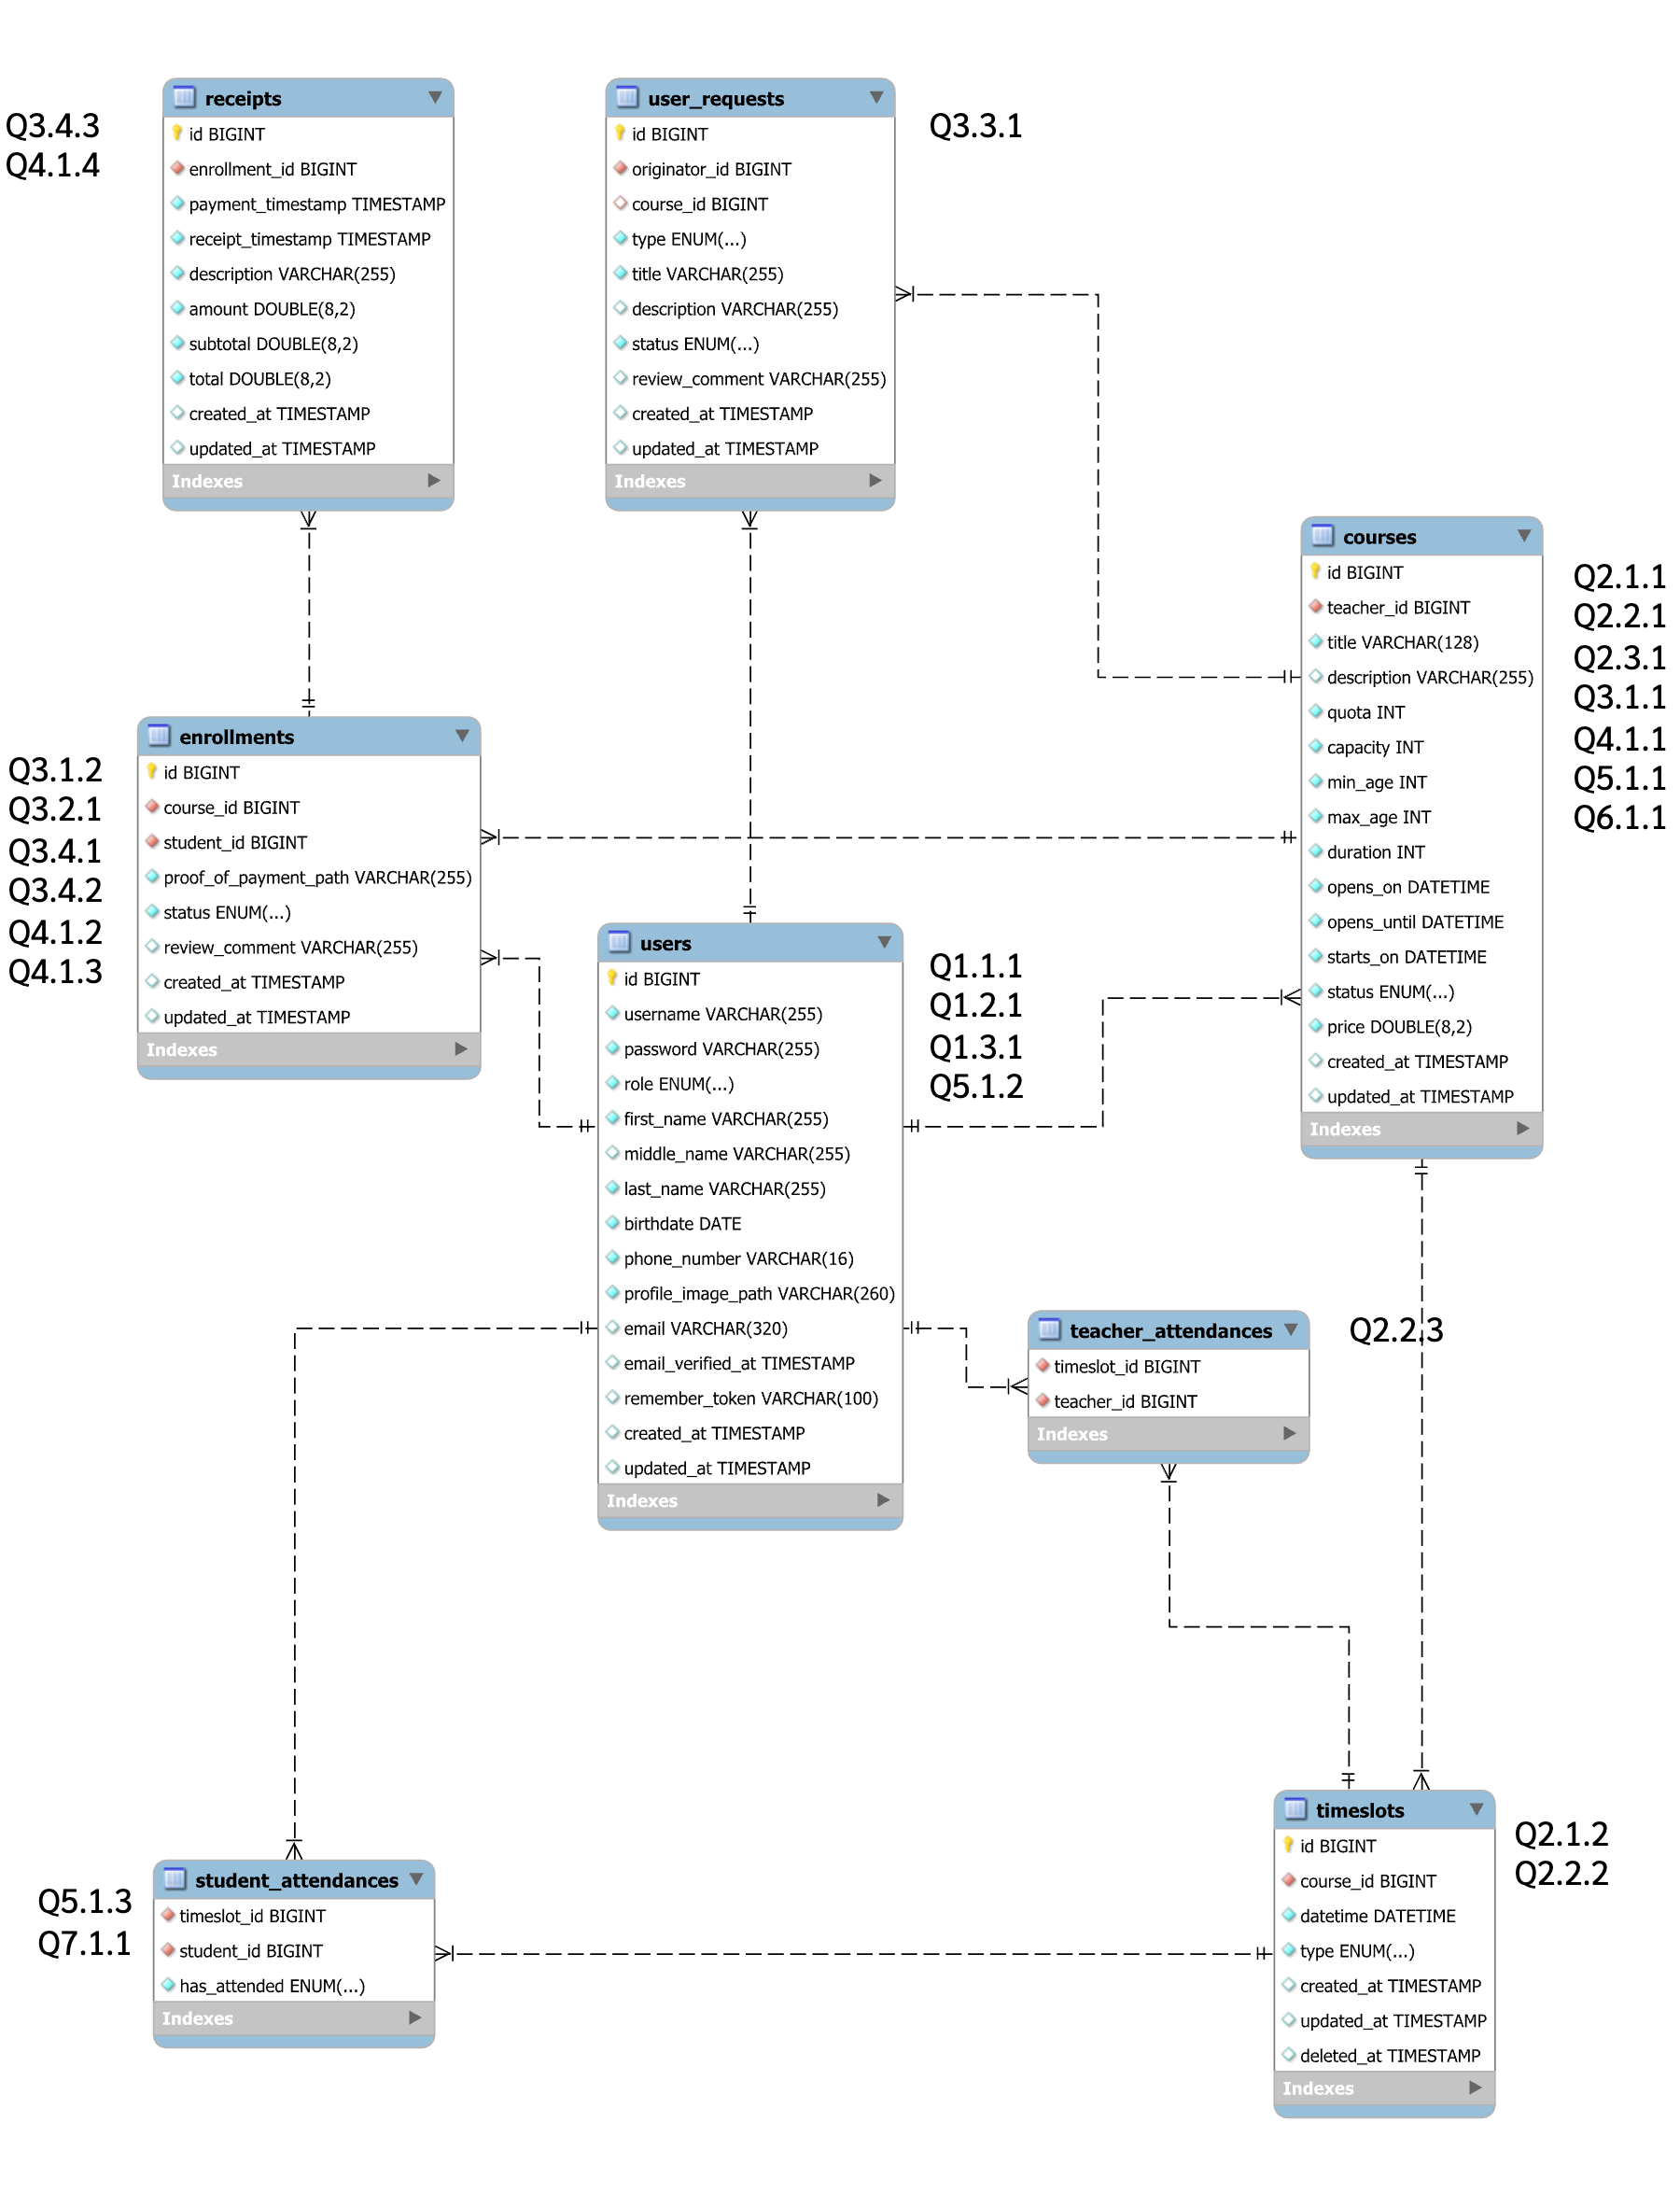
\includegraphics[width=\marginparwidth]{./figures/diagrams/entity-relationship/aqkids-entity-relationship-1.0.0-queries.png}}

\begin{landscape}
\subsubsection{Query Table}

\begin{table}[]
\caption{Query Table}
\label{tab:query-table}
\begin{tabularx}{\textwidth}{|l|l|l|l|}
\hline
\multicolumn{1}{|X|}{\textbf{Query ID}} & \multicolumn{1}{c|}{\textbf{Use Case ID}} & \multicolumn{1}{c|}{\textbf{Use Case}} & \multicolumn{1}{c|}{\textbf{SQL Query}}                                                                                                                                                                                                                                                                                                                                                                                                                                                        \\ \hline
Q1.1.1                                  & 1                                         & ยืนยันตัวตน                            & SELECT `username` FROM `users` WHERE `username` = USERNAME;                                                                                                                                                                                                                                                                                                                                                                                                                                    \\ \hline
Q1.2.1                                  & 1                                         & ยืนยันตัวตน                            & \begin{tabularx}{\textwidth}[X]{@{}l@{}}INSERT INTO `users` (\\ `username`,\\ `password`,\\ `role`,\\ `first\_name`,\\ `middle\_name`,\\ `last\_name`,\\ `birthdate`,\\ `phone\_number`,\\ `profile\_image\_path`,\\ `email`,\\ `created\_at`,\\ `updated\_at`) VALUES\\ (USERNAME,\\ PASSWORD,\\ ROLE,\\ FIRST\_NAME,\\ MIDDLE\_NAME,\\ LAST\_NAME,\\ BIRTHDATE,\\ PHONE\_NUMBER,\\ PROFILE\_IMAGE\_PATH,\\ EMAIL,\\ CREATED\_AT,\\ UPDATED\_AT);\end{tabularx}                                             \\ \hline
Q1.3.1                                  & 1                                         & ยืนยันตัวตน                            & SELECT `password` FROM `users` WHERE `username` = USERNAME;                                                                                                                                                                                                                                                                                                                                                                                                                                    \\ \hline
Q2.1.1                                  & 2                                         & จัดการคอร์ส                            & SELECT * FROM `courses`;                                                                                                                                                                                                                                                                                                                                                                                                                                                                       \\ \hline
Q2.1.2                                  & 2                                         & จัดการคอร์ส                            & SELECT * FROM `timeslots`;                                                                                                                                                                                                                                                                                                                                                                                                                                                                     \\ \hline
Q2.2.1                                  & 2                                         & จัดการคอร์ส                            & \begin{tabularx}{\textwidth}[X]{@{}l@{}}INSERT INTO `courses` (\\ `teacher\_id`,\\ `title`,\\ `description`,\\ `quota`,\\ `capacity`,\\ `min\_age`,\\ `max\_age`,\\ `duration`,\\ `opens\_on`,\\ `opens\_until`,\\ `starts\_on`,\\ `status`,\\ `price`,\\ `created\_at`,\\ `updated\_at`) VALUES\\ (TEACHER\_ID,\\ TITLE,\\ DESCRIPTION,\\ QUOTA,\\ CAPACITY,\\ MIN\_AGE,\\ MAX\_AGE,\\ DURATION,\\ OPENS\_ON,\\ OPENS\_UNTIL,\\ STARTS\_ON,\\ STATUS,\\ PRICE,\\ CREATED\_AT,\\ UPDATED\_AT);\end{tabularx} \\ \hline
Q2.2.2                                  & 2                                         & จัดการคอร์ส                            & \begin{tabularx}{\textwidth}[X]{@{}l@{}}INSERT INTO `timeslots` (\\ `course\_id`,\\ `datetime`,\\ `type`,\\ `created\_at`,\\ `updated\_at`,\\ `deleted\_at`) VALUES\\ (COURSE\_ID,\\ DATETIME,\\ TYPE,\\ CREATED\_AT,\\ UPDATED\_AT,\\ DELETED\_AT);\end{tabularx}                                                                                                                                                                                                                                           \\ \hline
Q2.2.3                                  & 2                                         & จัดการคอร์ส                            & \begin{tabularx}{\textwidth}[X]{@{}l@{}}INSERT INTO `teacher\_attendances` (\\ `timeslot\_id`,\\ `teacher\_id`) VALUES\\ (TIMESLOT\_ID,\\ TEACHER\_ID);\end{tabularx}                                                                                                                                                                                                                                                                                                                                        \\ \hline
Q2.3.1                                  & 2                                         & จัดการคอร์ส                            & UPDATE `courses` SET `status` = STATUS;                                                                                                                                                                                                                                                                                                                                                                                                                                                        \\ \hline
Q3.1.1                                  & 3                                         & สมัครคอร์ส                             & SELECT * FROM `courses`;                                                                                                                                                                                                                                                                                                                                                                                                                                                                       \\ \hline
Q3.1.2                                  & 3                                         & สมัครคอร์ส                             & SELECT * FROM `enrollments`;                                                                                                                                                                                                                                                                                                                                                                                                                                                                   \\ \hline
Q3.2.1                                  & 3                                         & สมัครคอร์ส                             & \begin{tabularx}{\textwidth}[X]{@{}l@{}}INSERT INTO `enrollments` (\\ `course\_id`,\\ `student\_id`,\\ `proof\_of\_payment\_path`,\\ `status`,\\ `review\_comment`,\\ `created\_at`,\\ `updated\_at`) VALUES\\ (COURSE\_ID,\\ STUDENT\_ID,\\ PROOF\_OF\_PAYMENT\_PATH,\\ STATUS,\\ REVIEW\_COMMENT,\\ CREATED\_AT,\\ UPDATED\_AT);\end{tabularx}                                                                                                                                                             \\ \hline
Q3.3.1                                  & 3                                         & สมัครคอร์ส                             & \begin{tabularx}{\textwidth}[X]{@{}l@{}}INSERT INTO `user\_requests` (\\ `originator\_id`,\\ `course\_id`,\\ `type`,\\ `title`,\\ `description`,\\ `status`) VALUES\\ (ORIGINATOR\_ID,\\ COURSE\_ID,\\ TYPE,\\ TITLE,\\ DESCRIPTION,\\ STATUS);\end{tabularx}                                                                                                                                                                                                                                                \\ \hline
Q3.4.1                                  & 3                                         & สมัครคอร์ส                             & SELECT * FROM `enrollments` WHERE `id` = ID;                                                                                                                                                                                                                                                                                                                                                                                                                                                   \\ \hline
Q3.4.2                                  & 3                                         & สมัครคอร์ส                             & UPDATE `enrollments` SET `STATUS` = STATUS, `review\_comment` = REVIEW\_COMMENT;                                                                                                                                                                                                                                                                                                                                                                                                               \\ \hline
Q3.4.3                                  & 3                                         & สมัครคอร์ส                             & \begin{tabularx}{\textwidth}[X]{@{}l@{}}INSERT INTO `receipts` (\\ `enrollment\_id`,\\ `payment\_timestamp`,\\ `receipt\_timestamp`,\\ `description`,\\ `amount`,\\ `subtotal`,\\ `total`,\\ `created\_at`,\\ `updated\_at`) VALUES\\ (ENROLLMENT\_ID,\\ PAYMENT\_TIMESTAMP,\\ RECEIPT\_TIMESTAMP,\\ DESCRIPTION,\\ AMOUNT,\\ SUBTOTAL,\\ TOTAL,\\ CREATED\_AT,\\ UPDATED\_AT);\end{tabularx}                                                                                                                \\ \hline
Q4.1.1                                  & 4                                         & จัดการการชำระค่าคอร์ส                  & SELECT * FROM `courses`;                                                                                                                                                                                                                                                                                                                                                                                                                                                                       \\ \hline
Q4.1.2                                  & 4                                         & จัดการการชำระค่าคอร์ส                  & SELECT * FROM `enrollments`;                                                                                                                                                                                                                                                                                                                                                                                                                                                                   \\ \hline
Q4.1.3                                  & 4                                         & จัดการการชำระค่าคอร์ส                  & UPDATE `enrollments` SET `status` = ‘SUCCESS’ WHERE `student\_id` = ID;                                                                                                                                                                                                                                                                                                                                                                                                                        \\ \hline
Q4.1.4                                  & 4                                         & จัดการการชำระค่าคอร์ส                  & \begin{tabularx}{\textwidth}[X]{@{}l@{}}INSERT INTO `receipts` (\\ `enrollment\_id`,\\ `payment\_timestamp`,\\ `receipt\_timestamp`,\\ `description`,\\ `amount`,\\ `subtotal`,\\ `total`,\\ `created\_at`,\\ `updated\_at`) VALUES\\ (ENROLLMENT\_ID,\\ PAYMENT\_TIMESTAMP,\\ RECEIPT\_TIMESTAMP,\\ DESCRIPTION,\\ AMOUNT,\\ SUBTOTAL,\\ TOTAL,\\ CREATED\_AT,\\ UPDATED\_AT);\end{tabularx}                                                                                                                \\ \hline
Q5.1.1                                  & 5                                         & ลงชื่อเข้าคาบเรียน                     & SELECT * FROM `courses`;                                                                                                                                                                                                                                                                                                                                                                                                                                                                       \\ \hline
Q5.1.2                                  & 5                                         & ลงชื่อเข้าคาบเรียน                     & SELECT * FROM `user` WHERE `id` = ID;                                                                                                                                                                                                                                                                                                                                                                                                                                                          \\ \hline
Q5.1.3                                  & 5                                         & ลงชื่อเข้าคาบเรียน                     & UPDATE `student\_attendances` SET `status` = ‘TRUE’ WHERE `student\_id` = ID;                                                                                                                                                                                                                                                                                                                                                                                                                  \\ \hline
Q6.1.1                                  & 6                                         & ปรับปรุงตารางเวลา                      & \begin{tabularx}{\textwidth}[X]{@{}l@{}}INSERT INTO `courses` \\ `timeslot\_id`,\\ `student\_id`) VALUES\\ (TIMESLOT\_ID,\\ STUDENT\_ID);\end{tabularx}                                                                                                                                                                                                                                                                                                                                                      \\ \hline
Q7.1.1                                  & 7                                         & รับ Certificate                        & \begin{tabularx}{\textwidth}[X]{@{}l@{}}SELECT COUNT(*) FROM `student\_attendances` WHERE `student\_id` = (SELECT `id` FROM `enrollments` WHERE `student\_id` = STUDENT\_ID)\\ AND `course\_id` = COURSE\_ID;\end{tabularx}                                                                                                                                                                                                                                                                                  \\ \hline
\end{tabularx}
\end{table}
\end{landscape}

\subsubsection{Table Structure}

\subsubsection{Use Case Description, Sequence Diagram, และ Collaboration Diagram}

\paragraph{Use Case 1}

\subsubsection{State Diagram}

\subsubsection{Class Diagram}

\subsubsection{Component Diagram}

\subsubsection{Site Map/User Interface Structure ของ Staff}

\subsubsection{Site Map/User Interface Structure ของ Teacher}

\subsubsection{Site Map/User Interface Structure ของ Student}
